\documentclass[onecolumn, draftclsnofoot,10pt, compsoc]{IEEEtran}
\usepackage{graphicx}
\usepackage{subcaption}
\usepackage{url}
\usepackage{setspace}
%\usepackage{hyperref}

\usepackage{geometry}
\geometry{textheight=9.5in, textwidth=7in}

% 1. Fill in these details
\def \CapstoneTeamName{		100k Challenge CS}
\def \CapstoneTeamNumber{		42}
\def \GroupMemberOne{			Michael Elliott}
\def \GroupMemberTwo{		 	Sam Hudson}
\def \GroupMemberThree{			Glenn Upthagrove}
\def \CapstoneProjectName{		100K Spaceport America Demonstration Rocket Project }
\def \CapstoneSponsorCompany{	School of MIME}
\def \CapstoneSponsorPerson{		Nancy Squires}

% 2. Uncomment the appropriate line below so that the document type works
\def \DocType{		Technology Review
				%Requirements Document
				%Technology Review
				Design Document
				%Progress Report
				}
			
\newcommand{\NameSigPair}[1]{\par
\makebox[2.75in][r]{#1} \hfil 	\makebox[3.25in]{\makebox[2.25in]{\hrulefill} \hfill		\makebox[.75in]{\hrulefill}}
\par\vspace{-12pt} \textit{\tiny\noindent
\makebox[2.75in]{} \hfil		\makebox[3.25in]{\makebox[2.25in][r]{Signature} \hfill	\makebox[.75in][r]{Date}}}}
% 3. If the document is not to be signed, uncomment the RENEWcommand below
%\renewcommand{\NameSigPair}[1]{#1}

%%%%%%%%%%%%%%%%%%%%%%%%%%%%%%%%%%%%%%%
\begin{document}
\begin{titlepage}
    \pagenumbering{gobble}
    \begin{singlespace}
    	
\includegraphics[height=4cm]{coe_v_spot1} %HERE
        \hfill 
        % 4. If you have a logo, use this includegraphics command to put it on the coversheet.
        %\includegraphics[height=4cm]{CompanyLogo}   
        \par\vspace{.2in}
        \centering
        \scshape{
            \huge CS Capstone \DocType \par
            {\large\today}\par
            \vspace{.5in}
            \textbf{\Huge\CapstoneProjectName}\par
            \vfill
            {\large Prepared for}\par
            \Huge \CapstoneSponsorCompany\par
            \vspace{5pt}
            {\Large\NameSigPair{\CapstoneSponsorPerson}\par}
            {\large Prepared by }\par
            Group\CapstoneTeamNumber\par
            % 5. comment out the line below this one if you do not wish to name your team
            %\CapstoneTeamName\par 
            \vspace{5pt}
            {\Large
                \NameSigPair{\GroupMemberOne}\par
                \NameSigPair{\GroupMemberTwo}\par
                \NameSigPair{\GroupMemberThree}\par
            }
            \vspace{20pt}
        }
        \begin{abstract}
        % 6. Fill in your abstract    
	The software suite developed for the American Institute of Aeronautics and Astronomic (AIAA) Spaceport America 100k Rocketry challenge for Oregon State University shall track a rocket as it flies. The resulting data will be used to both visualize the flight path and collect the rocket upon return to the surface. The software shall collect, filter, log, and visualize the data. This document describes the design of these systems. 
        \end{abstract}     
    \end{singlespace}
\end{titlepage}
\newpage
\pagenumbering{arabic}
\tableofcontents
% 7. uncomment this (if applicable). Consider adding a page break.
%\listoffigures
%\listoftables
\clearpage

% 8. now you write!
\section {Overview}
\subsection {Scope}
The following shall describe the design for the software that shall track the high altitude rocket for Oregon State University. The software shall primarily be running on the rocket, and a ground station. The data shall be collected from the sensors on the rocket, and begin a journey down a software pipeline towards final display, which will filter the data, package it, transmit it, collect it, covert it to a readable format, log it, and display it in both 2D and 3D displays. 
\subsection {Purpose} 
This software suit is intended to give reliable tracking of a rocket in flight, and graphically represent this data to the user. The general goals being the safe recovery of the rocket after it has completed its flight and come to rest. This is necessary as the rocket in this case shall go well outside of visible range, and the use of automated tracking shall be essential to the recovery. 
\subsection {Intended Audience}
The intended audience for this document are the engineering students responsible for the creation and use of the rocket, as well as their advisors. All involved are educated individuals, with a wide variety of expertise. Some have a very solid understanding of computer science whilst other have very different ares of expertise. This document provides sufficient description and detail for the most familiar of these stakeholders to understand most of the underlying systems, and a high enough view of the project and the connections for the readers of different background to still understand the purpose and general concepts behind the system. 
\section{Kalman Filter}
Author: Michael Elliott\\
One of the most challenging aspects of sending a rocket 100,000 feet
in the air is the collection and interpretation of accurate data from
the sensors.
At such high speeds and low pressure, there will be a lot of noise in the data.
We will need to collect and utilize the data we receive from the
sensors even though it may be inaccurate.
This means that we need a way to remove the noise from the readings.
In order to achieve this goal, we plan on using a Kalman filter.
A Kalman filter is an algorithm that uses linear quadratic estimation
to filter out statistical noise.
A Kalman filter uses a model to make predictions for the future state,
and adjusts those predictions based on input.
It begins with a known state, and compares each new input value to the
ideal predicted value.
It weights the predictions and the inputs to reach a reasonable middle
ground based on how much noise there is expected to be in the inputs.
The predictions are made based entirely on the current state and the
internal model for the behaviour.
This means that a Kalman filter can be run in real time.
It also means that it can be run on limited resources provided the
state and model are not overcomplicated.
Our Kalman Filter will be receiving input from at least a GPS, a
barometer, an accelerometer, a magnetometer, and a gyroscope.
The GPS provides latitude, longitude, and altitude.
The barometer provides atmospheric pressure.
The accelerometer provides acceleration.
The magnetometer provides orientation relative to the magnetic field
of the earth using three orthogonal sensors measuring the ambient
magnetic field.
The gyroscope provides angular velocity.
Internally, our state will keep track of the latitude, longitude,
altitude, polar angle, azimuthal angle, velocity, acceleration, jerk,
and rotation of the rocket.
Since the GPS readings are very accurate, a very high weight is going
to be given to those measurements.
Unfortunately, GPS has a hard time locking on at trans-sonic and
supersonic speeds, so chances are we will not get any GPS readings for
a significant portion of the flight.
The barometric pressure readings will be used to supplement our
altitude measurements.
Since at supersonic speeds the pressure readings will be much less
accurate, a lower weight will be given to them above a yet to be
determined velocity.
Likewise, the accelerometer, provides much noisier data at trans-sonic
and supersonic speeds.
This means that we will be highly reliant on the model and predictions
during supersonic flight.
This is especially important because we will be basing our velocity
and position calculations almost entirely on our acceleration
approximation at supersonic speeds.
Once the rocket slows down, we hope to get a GPS lock for a more
accurate reading of the position at apogee.
Another problem that the Kalman filter will help solve is if the
sensors show that the rocket is descending before due to noise it has
reached apogee.
This will prevent us from, for example, accidentally deploying our
parachutes early.
This Kalman filter will be part of the C code embedded on the rocket
and is the layer between the raw sensor data and the filtered results
exposed to the rest of the rocket and transmitted to the base station.
The input from the sensors will be raw input provided on pins from the PCB.
The Kalman filter will be its own module, providing an interface to
the rest of the rocket control to read the current rocket state from
it.
It will only expose a selection of the variables tracked within the
state to the rest of the program.
Additionally, the filter itself will be unmodifiable from the outside.
Given the extensive testing that will have to be done, a preliminary
Kalman filter will be completed by the end of December 2017.
This will be a basic filter that can be unit tested early to discover
any inconsistencies.
It will also allow us to test the other modules of our program before
the filter has been tailored to our needs.
Once we have the physical board on which the filter will be run, we
will be able to tailor the filter to our purposes.
We hope to have created working state transition and weight matrices
for the filter by the middle of March 2018.
This will leave us enough time to perform extensive integration
testing and tweak the coefficient matrices as necessary.
\section {Transmission Protocol}
Author: Michael Elliott\\
While travelling at high velocity over 20 miles in the air, the
atmosphere will be thin and there may be RF interference.
Even at such high speeds and long distances with a less than ideal
transmission medium, we still have to ensure ensure that the data
received by the ground station from the rocket is uncorrupted and that
it is received in the correct order.
In thinner atmosphere and at speeds over Mach 1, especially with
potential interference from the body of the rocket itself, there is
potential for high packet loss.
Due to an assumed high rate of packet loss as well as a lack of spare
processing power on the rocket, we will be unable to acknowledge the
receipt of packets and re-transmit a dropped packet if necessary.
This is why a protocol that assumes packets will be lost and can
compensate for the missing packets is required.
Since we can check the data integrity on the receiving end and drop
corrupt packets or interpolate missing ones, we don't have to worry
about a few corrupt or missing packets.
Despite this ability, we still want to minimize packet loss while also
minimizing processor use, so redundant transmission and reception
devices would be preferred.
Since the ground station will have plenty of spare processing power
when compared to the rocket, we can get away with very small packets.
As of right now, we plan on using 20 byte packets.
On a 32-bit processor, that will take 5 transmission cycles to fully
transmit the packet.
Keeping the amount of CPU time spent transmitting packets to a minimum
is ideal, so sticking to 20 byte packets will help us achieve this
goal.
With our current plans for the ground station, the only required data
is the latitude, longitude, altitude, and velocity.
We will also be including a time stamp in each packet.
The ground station software may display other information, but that
can all be derived from the provided data.
The transmission end of the protocol needs to be as lightweight as
possible, so we plan on simply sending out packets at a regular
interval on our radio frequency.
Once again, the bulk of the processing of the packets will be done on
the ground station, so all of the packet ordering, corruption
analysis, and interpolation will be performed there.
The transmission code will be part of the C code embedded on the
rocket and is what ensures the filtered data reaches the ground.
The transmission code will be its own module that interfaces with the
Kalman filter to read the state of the rocket and then interfaces with
the radio over SPI or IIC to send the data.
A preliminary version of the transmission code will be completed by
the end of December 2017 in order to facilitate proper testing.
This will allow us to unit test early and discover any inconsistencies.
It will also allow us to test how it works with the Kalman filter and
other modules of the program before the hardware is available.
Once we have the physical board on which the code will be run, we will
need to do more testing with that radio and with the ground station to
confirm that we can still receive a signal at a distance of 20 miles
or more.
We hope to have a fully functional transmission protocol by the middle
of March 2018.
This will leave us enough time to test our protocol in more extreme
conditions to ensure it is working how we expect.
The receiving side on the ground station is on a similar timeline.
We hope to have preliminary reception code ready by the time we have
the physical hardware that the transmission code is running on.
This way we will be able to test them both simultaneously.
\section{Packet Processing}
Author: Michael Elliott\\
Because of the potential for high packet loss and corruption, and the
small packet size, it will be necessary to process the packets on the
receiving end to use them effectively.
Firstly, all of the packets will be read from the radio and logged in
their raw form.
This will be handled by another module.
Then the packets will be passed on to the packet processor.
All of the packets have a timestamp, so the receiver will order the
received packets by the time sent to ensure they are processed in the
correct order.
The receiver will do a sanity check to make sure the timestamp did not
get corrupted in transit.
If the timestamp is corrupted, the entire packet will be discarded.
Otherwise the latitude, longitude, altitude, and speed will be
extracted from the packet.
At this point, a sanity check will be performed to ensure that none of
these values have been corrupted.
If a value has been corrupted, it will be discarded, however all other
values will be kept.
The discarded values will be interpolated using the values in the
preceding packets.
The interpolation will be done by using a quadratic best fit line for
the position and using the derivative of the position best fit line to
interpolate the speed.
Since the interpolation is predictive, the best fit line will use the
interpolated value as an additional sanity check for the data.
The packet processor will also use position data to augment the speed
data with the direction vector.
This way the packet processor will be able to expose reliable data to
the other components at their required rate regardless of when packets
are received.
It will also be able to retroactively update a component if a real
value is received after an interpolated value is provided by exposing
the entire history to the other modules.
Other modules will also be able to read all of the future interpolated
data points.
These techniques will minimize the impact of poor transmission
performance on the other components on the ground station.
The packet processor will be its own module that communicates with the
radio receiver module and the data visualization modules.
The packet processor will be completed after the preliminary
transmission code has been written in order to better understand our
needs.
This means that development for the packet processor will begin in mid
January of 2018, and the prototype code should be done in the next 4
weeks.
Following the development of the prototype, we will be able to do
extensive unit testing and integration testing with the other modules.
The packet processor is independent from the transmission protocol, so
it can be completed before the transmission code is finished.
This means that we should have the packet processor finished by March
2018, with additional testing to be performed upon the completion of
the other modules.
This module is the glue between the radio receiving data from the
rocket and all of the other code on the ground station, so the
correctness of the code must be confirmed.
\section {Data Handling}
Author: Glenn Upthagrove \\
%\subsection {design}
The data handling module shall be an entire subsystem, which mixes several standalone modules, as their own binaries, spawned as processes, and linked together with pipes. The first module shall be written in C, and shall have two main functions, to gather data from the hardware, and to spawn and link the other processes together. The data shall be directly retrieved by C from memory, as is dictated by the electrical engineering side of the project. The data will then be cast as a structure, which will separate the data as a separate 32bit single precision floats. These floats will then be passed onto a Python process which shall convert the data into a JSON format utilizing the Python JSON library. The python shall then pass that JSON data down the pipeline, and back to the parent data handling module, which will hand it off to the logging module, which it shall also spawn and communicate with via a pipe. This shall loop for the duration of the flight. This system shall be using concepts learned from operating systems one, specifically process spawning, pipe communication, and file I/O in C. It will also incorporate designs and testing methods learned in the software engineering courses. \cite{refjson} \cite{refpython} 
%\subsection {Communication}
The data handling parent, its two children, and the hardware, shall be communication using a centralized model, in which the data handler sits in the middle, and communicates independently with the other three components, which do not talk to each other. This is a design decision made to keep encapsulation, to regulate the communication through one node, and to allow for easier and more robust process management in the C language, as compared to splitting the process management up into both C and Python. The data in total is traveling down a pipeline, from collection through the filter and onto transmission on the rocket, followed by collection in hardware, into the data handling module, through the JSON converter, and on into the visualization on the ground station. The logging sits next to the pipeline, but is not an integrated piece inside of it. 
%\subsection {Testing}
The logging and JSON conversion modules should be completed before the parent module, as it will allow for seamless integration of the already compiled and tested binaries into the process spawning sections. The completion of the JSON conversion should also be completed before the logging module, as this allows for better integration testing of these systems, since it will be handling the data earlier than the logging system shall be, and is more important tot the overall project, as it passes the data along the pipeline for the visualization modules to use. The unit tests for this are slightly more interesting than the logging module. The parent process will have to have each of its individual functions tested one by one, most likely inside the same module. The communication can be faked with fake modules that can pass back good and bad data. The JSON conversion module can be tested in the same manner as the logging system, where a fake parent passes in good and bad data. These three modules will need integration testing with each other, and the JSON converter will need integration testing with the visualization modules. All of these tests shall be created with a make test, and tested at each git push origin master call using Travis CI hooked into the repository.  
An overview of this design is seen in Figure 1. 

\begin{figure}[h]
    \centering
%    \begin{subfigure}[Figure 1a]{0.3\textwidth}
        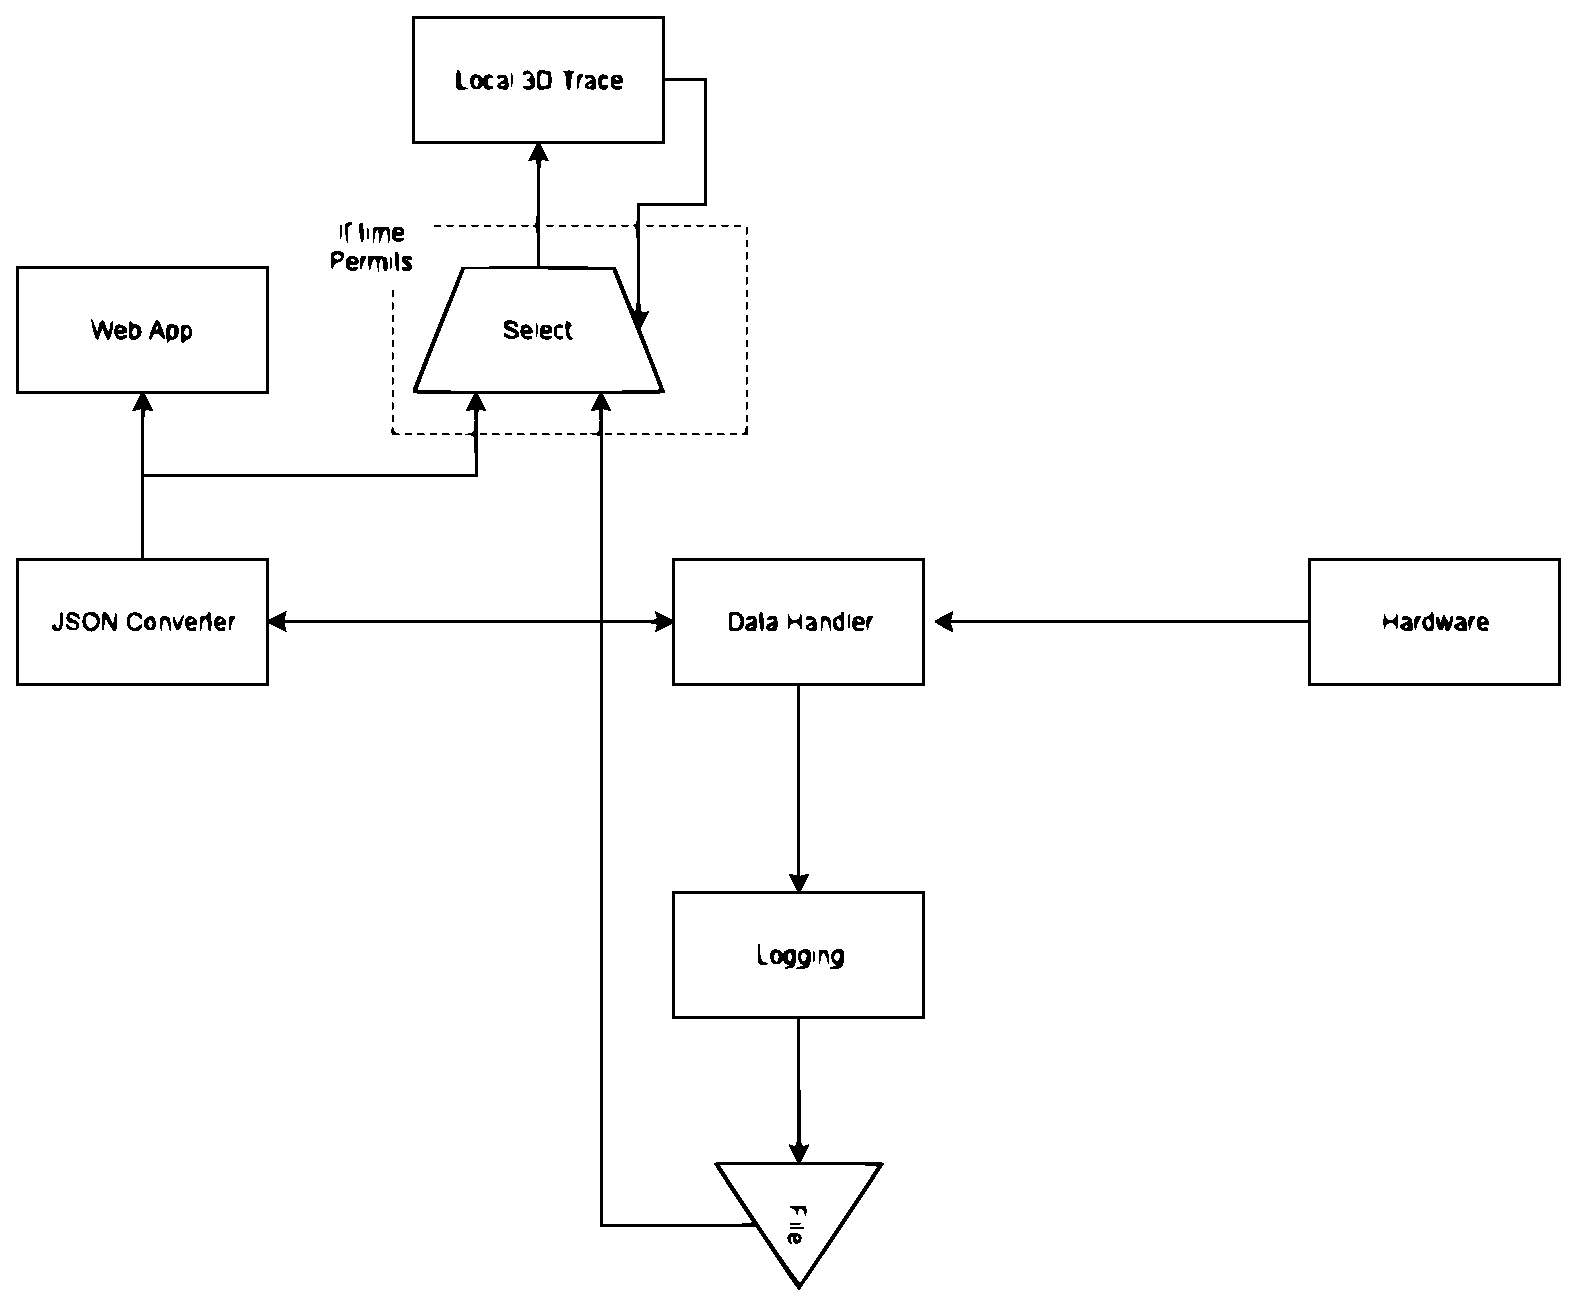
\includegraphics[height=8cm]{datahandel}
        \caption{A high level view of the Data Handling system and its interactions}
        \label{fig:handel}
%    \end{subfigure}
\end{figure}



\section {Logging}
Author: Glenn Upthagrove \\
%\subsection {Design}
The logging portion of this project shall sit inside the data handling module. The data handling module shall be the interaction with the hardware that collects the data from the hardware after receiving it from the antenna. The logging shall be a fairly simple component. Once the data is collected from hardware by a C module, the data will be converted into a JSON format by a Python module. Once the conversion is completed the data will be passed to alter portions of the pipeline, but also into the logging component. The component shall take in this data as a string. The module will then open a new .dat or .txt file if it is the first piece of data, if not, it will have the correct file already open. After this the data will be appended to the file. This will loop back up to the beginning and it will wait for the next piece of data. The logging component shall actually be its own process, communication with its parent, the data handling process, through a pipe. This is done because it gives timing for free. The logging process will write one data point, and then loop back to the top of its standard operations and wait for a new incoming piece of data, but instead of implementing any sort of complicated timing mechanism to wait for the next data point, it will simply hang until the pipe is filled with data again, which is given for free by the existing implementation of pipes. This allows the logging process to be kept simple, straightforward, and stable. \cite{refjson} \cite{refpython} 
%\subsection {Testing}
This module shall have several unit tests, which can be easily done by faking good and bad data. A fake parent process that creates fake data can be easily created to pass fake data in through the same pipe that will be used with the actual data handling module. This could be easily extended to random testing with a loop and random data generated by the fake parent. The random testing portion will pose a few extra challenges, as making fake bad data at random is simple, but creating good data is slightly harder. In mathematical terms, the set containing bad values has a far greater cardinality than that of the set of good data values. 
%\subsection {Tools}
The logging module shall be completed before the Data handling module. This will allow easier integration into the data handling module later, as the binary will already be compiled and tested before hand, and can be included in the new process spawning section immediately. This will allow the testing of the data handling module as a whole to be available at the same time as unit tests, immediately after completion. This section draws heavily from lessons learned in operating systems I and both software engineering classes. The file I/O for C that was taught in operating systems I is the fundamental knowledge required to create this module. The interaction between this module and its parent is also covered in this course, as it teaches process spawning and pipes. The testing required for this module are all covered in the second software engineering course, and those tools, specifically unit tests, shall be heavily implemented here.  
\section {Local 3D Trace}
Author: Glenn Upthagrove \\
%\subsection {Design}
The 3D trace will be a standalone system, created utiliziing OpenGL, which is an Application Programming Interface (API). The API shall be accessed through the a program written in the C++ language. The C++ language is fast, but also object oriented, allowing for abstraction and encapsulation of dome of the more complicated functions of the system. The program itself shall read in data from a file, which is in a JSON format, and then translate that data into vertices, each one representing the position of the rocket in one second intervals. The vertices shall be connected with a GL\_LINE\_STRIP topology. The ground shall be represented by a GL\_QUAD\_STRIP, making a large square plane, which shall then have a texture mapped to it of the area at which the launch is occurring. There shall be a preliminary module which reads in the file, converts it to a string, and then uses the string tokenizer function (strtok), to break it apart based off of the keys in the key value pairs for the JSON formatted flight data. This data shall be passed to a second module that converts the data into vertices, and connects them as a line strip, then stores this into a either a display list, or a vertex buffer object, depending on if the data was sufficiently large to justify the later. The third module would create a sufficiently large plane for representing the ground, reads in a .bmp file, converts it to a texture, and then maps the texture to the plane. The final step would be final display. Several libraries shall be utilized by this module, the OpenGL extension wrangler library (GLEW), and the OpenGL utility kit (glut). \cite{refopengl} \cite{refjson} 
%\subsection {Modes}
If time permits, a second mode will also be implemented, allowing data to come in through STDIN and be converted one vertex at a time, and update the trace in near real time, allowing for the tracking of the rocket in 3D during the flight. Also if time permits a sky box with a generic sky image could also be added, as well as the use of a vertex shader to transform the plane representing the ground based off of real topology data. Another addition would be the addition of and idealized model projected forwards based off of tall the data it had collected up until that point. Some of the tools used for the OpenGL programming will be tools provided by Professor Bailey of Oregon State University, which are being used with his express permission. 
%\subsection {Testing}
This system can be made at any time relative to the other modules, as it is a standalone system. It however would be preferable to finish the data handling system prior to the creation of this system, as the expansion of this with a near real time mode would be made far simpler if the system earlier in the pipeline that would send that data was already operational. Testing for this shall be done with a fake data creation process, which will create data using simple kinematic equations, and write them to a file for the 3D trace to then read and present. The file reading component can be tested individually with this file to see if the data read in matches. The vertex conversion component can be tested by logging all the data it is converting as it makes the vertices. The display portion can be tested by visual inspection when run, after the previous modules are proven to work sufficiently well. 
%\subsection {Tools} 
This creation of this system shall require th skills learned from computer graphics, as well as the introduction to computer science courses. The use of OpenGL as an API and correct manner in which to implement specific graphical elements come directly from the course work of introduction to computer graphics. The interaction of this API in C++, as well as the creation of a solid underlying system for handling the data comes from the C++ learned in the introductory courses. Data structures also lends a hand in the data handling first module, and the file I/O in that same module comes directly from Operating Systems I. 
An overview of design can be seen in Figure 2, where the left represents the near real time mode, and the right represents the post flight mode. 
\begin{figure}[h]
    \centering
%    \begin{subfigure}[Figure 1a]{0.3\textwidth}
        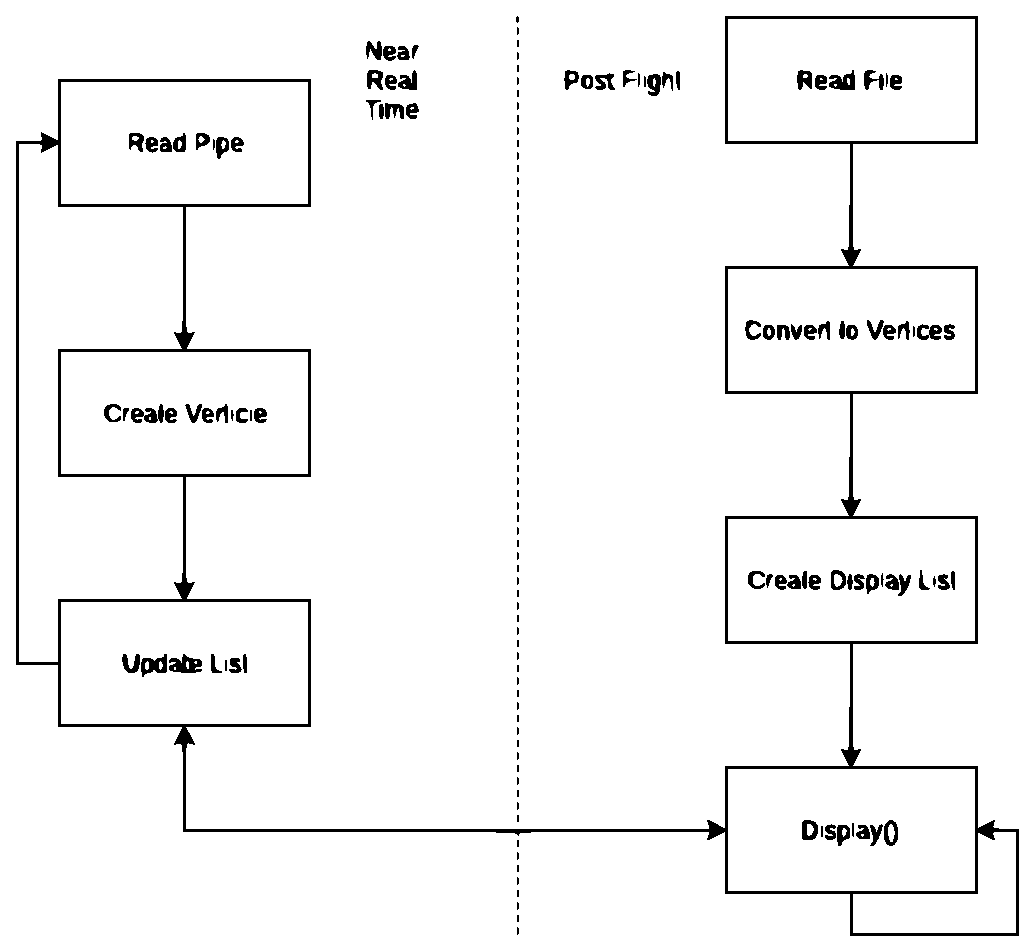
\includegraphics[height=8cm]{3DTrace}
        \caption{A high level view of the 3D Trace with both modes described}
        \label{fig:handel}
%    \end{subfigure}
\end{figure}
\section {Visualization}
Author: Sam Hudson\\
The open source JavaScript framework D3 will be used for rendering visualizations based on telemetry data received from the rocket. D3 is the best tool for creating these visualizations because it will allow for tight integration between data points making the visualizations more realistic. There will be three key visualizations. A speedometer for tracking the speed of the rocket throughout its flight, an altitude tracker used to track the rocket’s altitude in respect to the earth’s surface and a trajectory plotter which will plot an estimate of the trajectory based on existing telemetry data. The data used to render these visualizations will be in the form of a JSON object which will contain altitude, gps, velocity and timestamp data. Each visualization will be listening for new data added to the database (MongoDB) attached to the web application. This means that data visualizations can be updated in real time improving tracking and monitoring accuracy. All three visualizations will be displayed on the homepage of the web application to make for easy access. The speedometer visualization widget will utilize velocity data from each JSON object to represent the speed of the rocket throughout its flight. The speedometer will have two rates to represent speed; both mach and miles per hour. The altitude visualization widget will use the altitude data from each JSON object to position a 3D rocket object in a 3D space representing earth's surface and different layers of the earth’s atmosphere. This will give engineers tracking the rocket a better perspective of the rockets altitude in respect to the earth's surface. The altitude visualization will support zoom functionality which will allow users to pan further out relieving more layers or pan in to see the rocket in respect to a specific layer. A ruler will be positioned on the side of widget listing both miles and feet. The trajectory plotter visualization widget will be used to track the rockets position in real-time and also estimate its future position. This widget will make use of all elements of the data objects including, altitude, velocity, gps and time. The trajectory plotter visualization will contain a 3D globe object and a 3D rocket object. The rocket object in respect to the earth object is positioned based on the telemetry data stream. A trail will be also generated based on the rocket’s velocity. The trail will be color coded to indicate the level of acceleration at a given time. The colors will be categorized as follows: red indicates slower than existing average, yellow indicates inline with average and green indicates faster than average. Creating multiple listeners will allow for multiple asynchronous data streams. The listeners attached to each widget will receive data in an asynchronous fashion meaning data will be synchronized with the web page without requiring the page to be refreshed or interrupting the interactive experience. Each widget will be defined in separate JavaScript files to enhance maintainability. Using visualization tools to effectively track the rocket is a critical requirement to ensure the success of the mission. 
\section {Front-end}
Author: Sam Hudson\\
The front-end web framework Materialize will be used to design the web application. Materialize is a responsive frontend framework which will enhance user interactive experience and improve the overall interface design. Providing an intuitive and responsive user interface will make it trival for engineers to view important information about the rocket’s flight. The web application will be separated into five pages a main page, a page featuring the speedometer visualization, a page featuring the altitude visualization, a page featuring the trajectory plotter visualization and a page explaining more about the visualizations and how they work. The main page will contain a dashboard featuring all three visualizations widgets organized into three columns of width four. All pages will contain a navigation bar which features the AIAA logo, navigation elements and the current date and time. In addition all pages will feature a footer that will list copyright information and other additional information related to the organization. Splitting reusable code into separate files such as the navigation and footer makes maintaining the project a lot simpler. For example a changing the value of a HREF tag in an anchor element placed in the navigation would only require one update vs having to update each element on every page. This is a dynamic design technique which speeds up the development process. The materialize icon set will be used throughout the web application to improve usability. One benefit of using Materialize as a front-end framework is that it’s fully responsive. As the launch site will be remote it may be inconvenient to take larger devices. Adding adaptability for mobile web clients is essential. Materialize is very useful in that capacity by providing media CSS sets specific to different screen sizes. This works nicely in conjunction with D3. All graphics rendered by D3 are scalable vectors that respond well to changes in screen size. Another benefit of using Materialize as a frontend framework are the many built in mobile components. For example when the screen size becomes lower than a specific size, which can be defined at the discretion of the developer, an icon appears which reveals a collapsible mobile menu. In addition to rendered graphics on each visualization page there will also be tables listing different data values that are used in each data visualization. For instance, the altitude visualization page will have two columns for altitude and time. These tables will live under visualization widgets. To improve the efficiency of the web application both CSS and JS will be minified. The minification of CSS and JS will improve page loading time and reduce the total size of the project. Materialize makes it easy to integrate style changes. Common changes such as theme colors can be defined for all elements pretty simply in the main materialize CSS file. Materialize provides a lot of components that can be utilized. One useful component to have when loading content on a page is a preloader. Materialize had many determinate and indeterminate preloaders which can be useful to show the user that content is rendering. 
\section {Server-side}
Author: Sam Hudson \\
The server-side framework Flask-PyMongo will be used build the web application and API. Flask is a lightweight server side framework and PyMongo is a tool used for interacting the MongoDB. PyMongo is required because Flask doesn’t natively support Object Relational Models. As mentioned in the front-end development section the web application will consist of 5 pages. These five pages will contain widgets that rely on data contained within MongoDB. The main backend application will have 5 different routes: “main”, “altitude”, “speedometer”, “trajectory” and “about” these endpoints will be managed by handler functions that will be responsible for managing interactions with each page. Jinja2 is the templating engine that will be used to render each page. There will be three templates in total. One that will define the main page for the dashboard, one that will define the layout for the visualization pages and one that will define the about us page. Each handler function will gather related data for that specific page and pass that data into the jinja2 page rendering function. Data that’s specific to each page includes the page title, table contents, visualization widget data and current navigation information. An application programming interface will also need to be defined for access to data store in MongoDB. Two additional handler function will need to be defined for getting and setting telemetry data. The object model telemetry\_package will be defined with attributes: altitude, gps, velocity and timestamp. Making a get request to the telemetry\_package endpoint will return a list of all telemetry packages for use in D3 visualizations whereas the post endpoint will be responsible for adding telemetry packages to the database. Each call to the rest API will require a secure token which will be verified on the server. A function will be defined to authenticate and authorize selected transactions. This is an important security feature because it’s important to verify the sender is who they say there are. Authenticity can be validated because only systems with access to a secret token will be able to authenticate against the API. D3 visualizations will be defined in JavaScript and only interface with the API. Telemetry data will not be served through standard page handlers. Flask has a built in local development server which will suitable for hosting this web application and API. Only localized access is required the application will not be public facing. MongoDB is the best database technology for the specific case. Telemetry data will be stored as JSON objects. JSON Objects are the format in which MongoDB stores data within its database. This means little effort is required to store this data because data sent to the API will already be in the correct format to store within the database. MongoDB is a non-relational database that scales very well and can store large amounts of data. MongoDB is a high performance database technology that can handle many different requests.
\section {Connection Overview} 
The basic topology of the system in its entirety is a pipeline. At the beginning raw data comes in from the sensors, and at the other end is displayed in a meaningful way to the screen. There are of course a few pieces that do not fit perfectly into the pipeline model, the logging module and the local 3D trace for instance, but the main goal, and the modules meant to achieve it, fall fairly neatly into this topology. The first few stages are done on the rocket, where the data is collected, sent to a Kalman filter, packaged neatly and transmitted. These modules shall primarily be authored by Michael Elliott. The middle stage is where data is received by hardware on the ground station, collected from hardware, and converted to JSON. These modules shall primarily be authored by Glenn Upthagrove. The final stage, the visualization, receives the JSON data, goes through the web API, into a mango DB module, into the web application, and finally to the display. These components shall primarily be authored by Samuel Hudson. The logging module, the log file, and local 3D trace shall sit next to the main pipeline. The overview of the abstracted pipeline is illustrated in Figure 3. 
\begin{figure}[h]
    \centering
%    \begin{subfigure}[Figure 1a]{0.3\textwidth}
        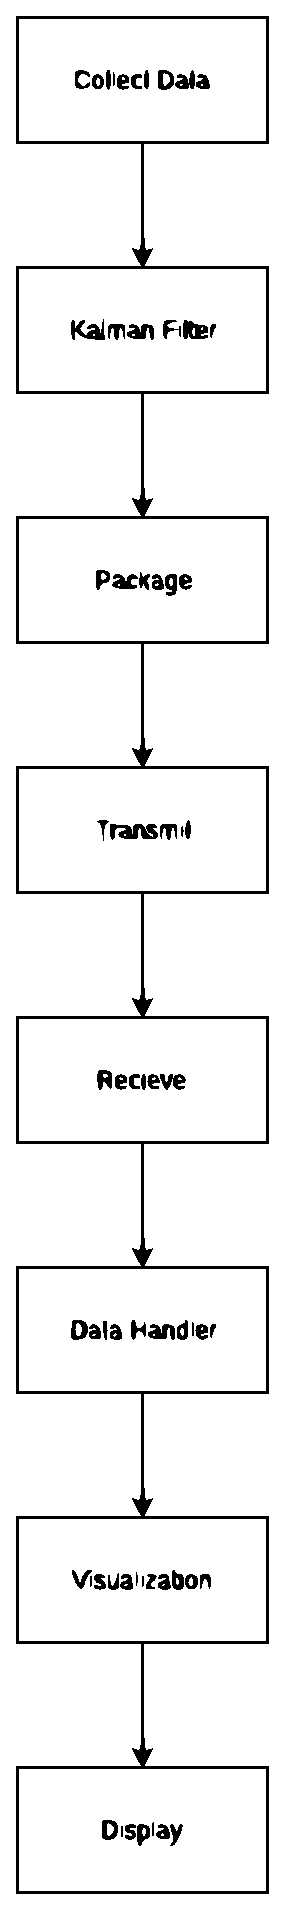
\includegraphics[height=12cm]{basicpipeline}
        \caption{An abstracted view of the software pipeline}
        \label{fig:handel}
%    \end{subfigure}
\end{figure}
\section {Conclusion}
All of these components will fit together into the final collection of
software used to track the rocket during flight.
This will help achieve the goal of reaching 100,000 feet of altitude.
Each component is an important cog in the overall machine, and they
all must fit together properly in order for us to succeed.
This is why having a well thought out design is so important for our project.
It ensures that all of the important pieces fit together well and
gives us a road map for our testing in the future.
With such a critical mission, there is very little tolerance for
error, so testing thoroughly and designing properly is paramount.

\bibliographystyle{IEEEtran}
\bibliography{bibliography}


\end{document}
